\chapter{Literature Review}
\label{chap-lr}
In this chapter, a comprehensive literature overview is provided. We start with a brief introduction to deep generative learning in Section \ref{sec-Deepgenerativelearning} and kernel-based learning in Section \ref{sec-kernelbasedlearning}. The basic theoretical formulation of Gen-RKM is then presented in Section \ref{sec-tfgenrkm}. Lastly, we review related works that address data imbalance in the context of both classification and generative learning in Section \ref{sec-learning-from-unbalanced-data}.
\section{Deep generative learning}
\label{sec-Deepgenerativelearning}
Deep generative learning has always been a fascinating frontier in the field of artificial intelligence for the last decade. The reason for that is its remarkable capability to generate almost indistinguishable synthetic samples from real-world objects. Generative models have diverse applications in the real world,  including painting creation, speech synthesis, language learning, and many others. Below we will discuss the difference between generative learning and traditional discriminative learning, as well as some state-of-the-art models in generative learning.

\subsection{Generative learning vs. discriminative learning}
\label{subsec-Generativelearningvsdiscriminativelearning}
The key distinction between generative approaches and discriminative approaches is their different underlying probability inference procedures. Mathematically speaking, given a dataset with feature-label pairs $\{\bx,\by\}$, discriminative learning is interested in modeling the conditional probability of $\by$ given feature $\bx$, namely $p(\by|\bx)$. In contrast with that, generative learning tends to capture the joint probability $p(\bx,\by)$, enabling it to generate new samples by random sampling from the learned distributions. Note that it is also very common to just model $p(\bx)$ in generative learning since the information on labels is not always available in practice. In general, generative models need to estimate the overall distribution of the data, whereas discriminative classifiers merely aim to find the optimal decision boundary in the data space. This fundamental distinction explains why training generative models is generally more computationally expensive than training discriminative models.


\subsection{State-of-the-art: VAEs and GANs}
\label{subsec-VAEGAN}
Generative learning has gone through significant advancements over recent decades thanks to the developments in deep neural network architectures, with various types of generative models emerging.  Among these, Variational Autoencoders (VAEs) and Generative Adversarial Networks (GANs) have achieved great success for their widespread adoption. Below, we provide a brief introduction to these two models. One can refer to \cite{xuOverviewDeepGenerative2015} for more detailed overviews on other types of generative models.

\noindent \textbf{Variational Autoencoders:} VAE is a type of latent variable model combining the probabilistic framework with an encoder-decoder architecture, first proposed by Kingma and Welling in 2013 \cite{kingmaAutoEncodingVariationalBayes2022}. Let input data be $\bx\in \mathcal{X}$ and latent variables be $\bz\in \mathcal{Z}$ with prior distribution $p(\bz)$ (usually pre-defined as a Gaussian distribution). Since the joint distribution $p_{\btheta}(\bx,\bz)$ is implicitly defined in VAE, the conditional distribution of $\bx$ given latent variable $\bz$ can be denoted as $p_{\btheta}(\bx|\bz)$ where $\btheta$ is the parameter vector. A natural parameters estimations procedure is via maximizing marginal log-likelihood of $\bx$, where
\begin{equation}
    \log p_{\btheta}(\bx) = \log \int p_{\btheta}(\bx|\bz)p(\bz)d\bz.
\end{equation}
However, optimizing on marginal log-likelihood is intractable because of the existence of an integral part. To tackle this problem, Kingma et al. proposed using evidence lower bound (ELBO) to approximate the exact marginal likelihood, which can be written as 
\begin{equation}
    \begin{aligned}
        \log p_{\btheta}(\bx) &= \log \int q_{\bphi}(\bz|\bx) \frac{p_{\btheta}(\bx|\bz)p(\bz)}{q_{\bphi}(\bz|\bx)}d\bz \\
        &\geq \int q_{\bphi}(\bz|\bx) \log \frac{p_{\btheta}(\bx|\bz)p(\bz)}{q_{\bphi}(\bz|\bx)} d\bz \\
        &= \E_{q_{\bphi}(\bz|\bx)} [\log p_{\btheta}(\bx|\bz) + \log p(\bz) - \log q_{\bphi}(\bz|\bx)] \\
        &= \underbrace{\E_{q_{\bphi}(\bz|\bx)}[\log p_{\btheta}(\bx|\bz)]}_{\text{log-likelihood}} - \underbrace{D_{KL}[q_{\bphi}(\bz|\bx) || p(\bz)]}_{\text{KL divergence}} = \mathcal{L}_{ELBO}.
    \end{aligned}
\end{equation}
$q_{\bphi}(\bz|\bx)$ is known as proposal distribution (or recognition model) to approximate the true prior and $p_{\btheta}(\bx|\bz)$ is often called generation model, corresponding to encoder and decoder part in VAE respectively. The first term (log-likelihood term) in the training objective can be approximated by 
\begin{equation}
    \E_{q_{\bphi}(\bz|\bx)}[\log p_{\btheta}(\bx|\bz)] \approx \frac{1}{N}\sum_{i=1}^{N}\log p_{\btheta}(\bx|\bz^{(i)})
\end{equation}
with $\{\bz^{(i)}\}_{i=1}^{N}$ sampled from proposal distribution $q_{\bphi}(\bz|\bx)$. Kingma et al. suggested using a reparameterization trick where $\bz^{(i)} = g_{\bphi}(\bx,\boldsymbol{\epsilon}^{(i)})$ with ${\epsilon}^{(i)} \sim \Normal(\boldsymbol{0},\boldsymbol{\text{I}})$. $g_{\bphi}(.)$ is a differentiable and deterministic function that ensures the differentiability of the stochastic sampling process, allowing gradient-based optimization schemes can be effectively used for training VAEs. 


\noindent \textbf{Generative Adversarial Networks:} GANs were first introduced by Goodfellow et al. in 2014 \cite{goodfellowGenerativeAdversarialNets2014}, bringing revolutionary impacts to the field of generative learning due to their exceptional ability to generate highly realistic images through adversarial training schemes. Unlike in VAE, GAN learns the underlying distribution of data without explicit density estimation, which means we do not have to parametrically pre-define the distribution of data. A GAN typically consists of two multilayer neural networks, namely a discriminator $\mathcal{D}: \bbR^{d} \to \{0,1\}$ and a generator $\mathcal{G}: \bbR^{l} \to \bbR^{d}$, where $d$ is the dimension of input data and $l$ is the dimension of latent space. Discriminator is simply a binary classifier that distinguishes real data from fake data (i.e. data generated by generator), whereas generator is for image synthesis given a noise input $\bz$. The general architecture of GAN is shown in figure \ref{GAN-schematic}. The training objective in vanilla GAN is written as 
\begin{equation}
    \min_{\mathcal{G}} \max_{\mathcal{D}} V(\mathcal{D}, \mathcal{G}) = \E _{\bx \sim p_{\mathcal{X}}(\bx)}[\log \mathcal{D}(\bx)] + \E_{\bz \sim p_{\mathcal{Z}}(\bz)}[\log(1-\mathcal{D}(\mathcal{G}(\bz)))],
    \label{ganobj}
\end{equation}
where probability of discriminator giving the right classification is maximized in the first expectation term while generator is trained to fool the discriminator. The whole optimization problem can be intuitively regarded as a min-max game with two players, each side wants to defeat the other. The global optimality of \ref{ganobj} has been proven to be $p_{\mathcal{X}}(\bx) = p_{\mathcal{G}}(\bx)$, which means the distribution of fake samples and the distribution of real samples are identical under optimality condition \cite{goodfellowGenerativeAdversarialNets2014}.

\begin{figure}[H]
    \centering
    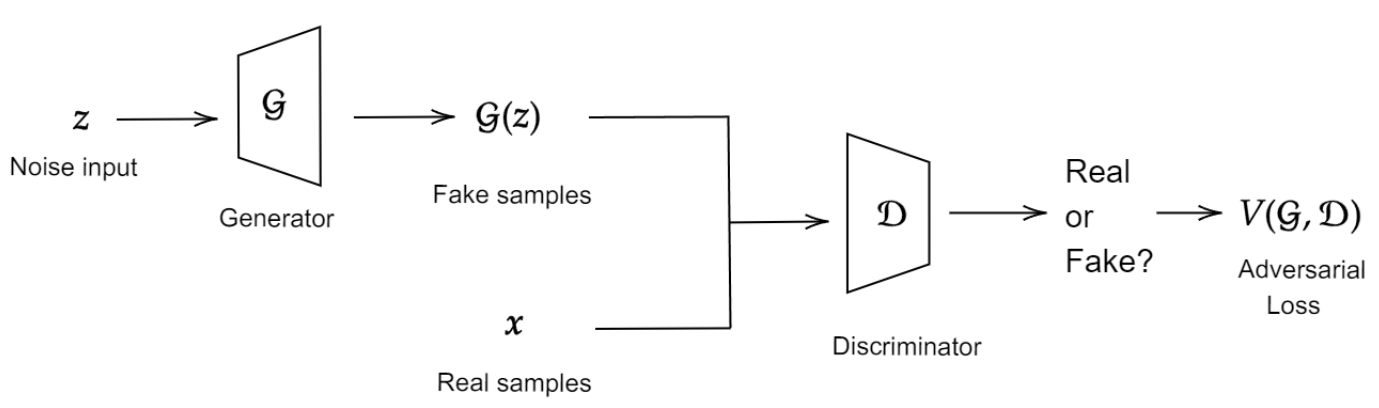
\includegraphics[width = 0.9\textwidth]{Figures/LR/GAN-schematics.png}
    \caption{Schematic diagram of vanilla GAN architecture}
    \label{GAN-schematic}
\end{figure}


\section{Kernel-based learning}
\label{sec-kernelbasedlearning}
Kernel methods were first introduced by Vapnik (1995), gaining great attention through their successful application onto Support Vector Machines (SVMs) \cite{vapnikNatureStatisticalLearning2000,cortesSupportvectorNetworks1995}. Kernel-based learning extends traditional linear approaches to non-linear scenarios by projecting input data into a high-dimensional feature space using a non-linear mapping function $\varphi(.)$. The core motivation behind that is one can expect linearly separable patterns in the feature map space, thus traditional linear techniques can learn more complex patterns from non-linear data after feature mapping. One great challenge is that features may lie in very high dimensions, possibly infinite, which makes computing $\varphi(.)$ very expensive or even intractable. 

Thanks to Mercer's theorem, it is possible to implement kernel methods without explicitly knowing the form of $\varphi(.)$ making them both powerful and computationally convenient. More precisely, given input data $\{\bx_i\}_{i=1}^{N}$ with $\bx \in \bbR^d$, Mercer's theorem states that there exists a feature mapping $\varphi: \bbR^d\to \caH$ and a kernel function $K: \bbR^d \times \bbR^d \to \bbR$ such that 
\begin{equation}
    K(\bx,\bz) = \varphi(\bx)^\top\varphi(\bz),
\end{equation}
if and only if $K(.,.)$ is a positive-definite function \cite{suykensLeastSquaresSupport2002}. The above theorem implies that kernel $K$ can be written as the dot product of two data points, and the collection of kernels on all pairs of training examples in the data set is defined as the kernel matrix (or Gram matrix) where 
\begin{equation}
\bK = \begin{bmatrix}
K(\bx_1, \bx_1) & K(\bx_1, \bx_2) & \cdots & K(\bx_1, \bx_N) \\
K(\bx_2, \bx_1) & K(\bx_2, \bx_2) & \cdots & K(\bx_2, \bx_N) \\
\vdots & \vdots & \ddots & \vdots \\
K(\bx_N, \bx_1) & K(\bx_N, \bx_2) & \cdots & K(\bx_N, \bx_N)
\end{bmatrix}.
\end{equation}
The computational problem can be then addressed by pre-computing the kernel matrix since the size of the kernel matrix is fixed on $N\times N$.
The general procedure of working on kernel matrix $\bK$ is usually referred to as \emph{kernel trick}.

Some representative applications of kernel methods in machine learning include Support Vector Machines (SVMs) \cite{cortesSupportvectorNetworks1995}, spectral clustering \cite{ngSpectralClusteringAnalysis2001}, Kernel Principal Component Analysis (KPCA) \cite{scholkopfKernelPrincipalComponent1997}, Gaussian Processes \cite{rasmussenGaussianProcessesMachine2004}, and etc. Beyond that, inspired by the powerful representation learning capabilities of deep learning architectures, there is growing interest in finding new synergies between traditional kernel methods and deep neural networks \cite{choKernelMethodsDeep2009, chenOverviewDeepKernel2016}. One notable example is Deep Restricted Kernel Machines (DRKM), which encapsulates KPCA, SVMs and possibly some other kernel learning techniques into one unified deep learning architecture via conjugate feature duality \cite{suykensDeepRestrictedKernel2017}. One can refer to \cite{hofmannKernelMethodsMachine2008,scholkopfLearningKernelsSupport2018}  for more detailed overviews and explanations on kernel-based learning.



\section{Theoretical framework of Generative restricted kernel machine}
\label{sec-tfgenrkm}
The theoretical framework of Generative restricted kernel machine (Gen-RKM) algorithm is discussed in this section. Starting by reviewing PCA and KPCA in subsection \ref{subsec-pcakpca}, the general restricted kernel machine (RKM) framework is then illustrated in subsection \ref{subsec-basicformulaRKM}. Next, subsection \ref{subsec-basicformulaGenRKM} showcases the basic training and generation algorithm of Gen-RKM under both single-view and multi-view scenarios. Besides, some related variants of Gen-RKM are introduced in subsection \ref{subsec-relatedvariantsofgenrkm}.

\subsection{A brief overviews on PCA and Kernel PCA}
\label{subsec-pcakpca}
\textbf{Basic formulation of PCA} \ Principal Component Analysis (PCA) is a widely-used unsupervised algorithm for dimensionality reduction while preserving as much variability as possible in the data \cite{bishopPatternRecognitionMachine2006, karamizadehOverviewPrincipalComponent2013}. Intuitively, PCA searches for a linear transformation such that maximizes the variance of the projected data in a lower-dimensional subspace. Orthonormal vectors that span this subspace after projection is often called \emph{principal components} (PCs). In the mathematical setting, one can formulate PCA as a constrained optimization problem. Consider a data matrix $\mathbf{X} = [\bx_1,\bx_2,\dots,\bx_N]\in \bbR^{d\times N}$ (here we assume data has already been centered for simplicity), the \emph{maximum variance formulation} \cite{bishopPatternRecognitionMachine2006} of PCA is given by 
\begin{equation}
    \begin{aligned}
        \max_{\bu_i} & \quad \bu_i^\top \mathbf{C} \bu_i \\
        \text{s.t}& \quad  \|\bu_i\|_2^2=\bu_i^\top \bu_i = 1,
    \end{aligned}
\end{equation}
where $\bu_i \in \bbR^d$ is the $i^{th}$ principal component and $\mathbf{C}$ is the sample covariance of the data ,defined as 
\begin{equation}
  \mathbf{C} = \frac{1}{N} \mathbf{X}\mathbf{X}^\top = \frac{1}{N} \sum_{n=1}^{N} \bx_{n}\bx_{n}^\top.
\end{equation}
Solving the Karush-Kuhn-Tucker (KKT) conditions of this constrained optimization problem, one can obtain the optimal conditions as the eigen-decomposition form on covariance matrix $\mathbf{C}$:
\begin{equation}
    \mathbf{C}\bu_i = \lambda_i\bu_i, \quad i=1,\dots, r.
    \label{PCA-solution}
\end{equation}
where $\lambda_i$ corresponds to the Lagrange multiplier. That indicates that the optimal principal components are the eigenvectors corresponding to the $r$ largest eigenvalues $\lambda_1, \dots, \lambda_r$ solved from eigen-decomposition problem. An alternative formulation of PCA is based on \emph{minimum reconstruction error} \cite{bishopPatternRecognitionMachine2006}. We denote a set of orthonormal directions as matrix $\mathbf{U} = [\bu_1,\bu_2, \dots, \bu_r]$, the reconstructed data point in PCA is simply $\tilde{\bx}_n = \mathbf{U}\mathbf{U}^{\top}\bx_n$, which leads to the following straightforward reconstruction error minimization problem:
\begin{equation}
    \begin{aligned}
        \min_{\mathbf{U}} & \quad \frac{1}{N}\sum_{n=1}^{N}\|\bx_n-\tilde{\bx}_n \|^2_2 \\
        \text{s.t}& \quad \mathbf{U}^\top \mathbf{U} = \mathbf{I}.
    \end{aligned}
    \label{PCA-recon-obj}
\end{equation}
It is easy to verify that the optimal solution for \ref{PCA-recon-obj} is equivalent to \ref{PCA-solution}. 

\noindent\textbf{Basic formulation of Kernel PCA} \ PCA is limited in only capturing the linear patterns in the data which makes it fail to generalize well on more complex non-linear data. Sch\"{o}lkopf et al. \cite{scholkopfKernelPrincipalComponent1997} extended the vanilla PCA algorithm to a non-linear setting based on kernel methods. Consider a non-linear mapping function $\bphi(.): \bbR^d\to \mathcal{H}$, the basic idea of kernel principal component analysis (KPCA) is to perform conventional PCA on the mapped data in the feature space. The sample covariance matrix after feature map now becomes 
\begin{equation}
    \mathbf{C}_{\bphi} = \frac{1}{N} \sum_{n=1}^{N} \bphi(\bx_{n})\bphi(\bx_{n})^\top = \frac{1}{N} \bPhi \bPhi^\top,
    \label{KPCA-eigen-decop}
\end{equation}
and its corresponding eigen-decomposition problem is given by
\begin{equation}
 \mathbf{C}_{\bphi}\bu_i = \lambda_i\bu_i, \quad i=1,\dots, r.
\end{equation}
where $\bPhi = [\bphi(\bx_1),\bphi(\bx_2),\dots,\bphi(\bx_N)]$. We usually refer to the formulation of eigen-decomposition on covariance matrix as the \emph{primal} form because function $\bphi(.)$ needs to be explicitly defined under this case. To avoid directly working on explicit feature map function $\bphi(.)$, Sch\"{o}lkopf et al. reformulated this problem by cleverly using integral operator kernel functions \cite{scholkopfKernelPrincipalComponent1997}. Starting from equation (\ref{KPCA-eigen-decop}), an equivalent form can be achieved by multiplying $\bphi(\bx_l)^\top (l = 1,\dots,N)$ on both sides : 
\begin{equation}
    \bphi(\bx_l)^\top\cdot \frac{1}{N} \sum_{n=1}^{N} \bphi(\bx_{n})\bphi(\bx_{n})^\top\bu_i = \lambda_i(\bphi(\bx_l)^\top\cdot\bu_i).
    \label{KPCA-dual-init}
\end{equation}
Moreover, one can write the eigen-vectors $\bu_i$ in the form of linear combination of $\bphi(\bx)$ where
\begin{equation}
    \bu_i = \sum_{m=1}^N h_{im}\bphi(\bx_m).
    \label{KPCA-lc-pc}
\end{equation}
Combining equations (\ref{KPCA-lc-pc}) with (\ref{KPCA-dual-init}), the key eigenvector equation can be expressed in terms of kernel function $K(\bx_i,\bx_j) = \bphi(\bx_i)\top \bphi(\bx_j)$ : 
\begin{equation}
    \frac{1}{N} \sum_{n=1}^{N} K(\bx_l,\bx_n) \sum_{m=1}^{N} h_{im} K(\bx_n,\bx_m) = \lambda_i \sum_{m=1}^{N} h_{im} K(\bx_l,\bx_n).
\end{equation}
After simplifying, one can obtain a neat expression 
\begin{equation}
    \bK\bh_i = \lambda_i N \bh_i
    \label{KPCA-dual-obj}
\end{equation}
where coefficients vector $\bh_i = [h_{i1},h_{i2},\dots, h_{im}]^\top$ and $\bK$ is the gram matrix of kernel function $K(.,.)$. It is obvious that equation (\ref{KPCA-dual-init}) is exactly the eigen-decomposition problem on kernel matrix $\bK$, hence one can solve the KPCA problem given a high dimensional feature space without demanding computational costs. Notice that when a linear kernel function is provided, KPCA will be reduced to conventional PCA.

\noindent\textbf{LS-SVM formulation of Kernel PCA} \ Least Squares Support Vector Machine (LS-SVM) is a modification on the formulation of the original SVM optimization problem introduced by Suykens et al. \cite{suykensLeastSquaresSupport1999,suykensLeastSquaresSupport2002}. The key difference between LS-SVM formulation and basic SVM formulation is in two-fold. First, inequality constraints in SVM is translated to equality constraints by introducing an error variable $\be_i$. Secondly, a squared loss term on $\be_i$ is included in the objective converting quadratic programming (QP) problem to solving a set of linear equations \cite{suykensLeastSquaresSupport2002}. The computation is greatly simplified thanks to LS-SVM form while most of key advantages of traditional SVM are preserved,  such as the primal-dual representation \cite{suykensPrimalDualModel2010}. 

Not limited to SVM classifiers, LS-SVM also provides an alternative formulation for KPCA that can be written as
\begin{equation}
    \begin{aligned}
            \min_{\mathbf{W}, \be_i}& \quad \frac{\eta}{2}\bW^\top\bW - \frac{1}{2}\sum_{i=1}^{N}\be_{i}^\top \Lambda^{-1} \be_{i}  \\
    \text{s.t}& \quad \be_i = \bW^\top \bphi(\bx_i) \quad \forall i =1,\dots,N
    \label{LSSVM-KPCA-OBJ}
    \end{aligned}
\end{equation}
with $\Lambda = \text{diag}(\lambda_1,\dots,\lambda_r)$ and transformation matrix $\bW$. This optimization problem is analogous to one class modeling problem in the context of SVM where only a zero target value is considered. One can recover the optimal solution to the eigen-problem on kernel matrix $\bK$ (equation (\ref{KPCA-dual-obj})) by solving the KKT conditions. In case $\bphi(\bx)$ is not zero-mean, centering before performing PCA is nontrivial. The error variable (or score variable) in problem (\ref{LSSVM-KPCA-OBJ}) then becomes $\quad \be_i = \bW^\top (\bphi(\bx_i) - \boldsymbol{\mu_{\bphi}})$ \cite{suykensLeastSquaresSupport2002}.


\noindent\textbf{Preimage problem in Kernel PCA} \ One important use case in KPCA is denoising, i.e. removing unwanted noisy patterns by projecting training data onto subspace spanned by eigenvectors. Furthermore, denoising requires mapping the projected data back to the original input space, namely reconstructing the data. Reconstruction in linear PCA is straightforward because only simple matrix multiplication is involved. However, reconstructing data in Kernel PCA is way more complicated due to the implicit nature of feature map function $\bphi(.)$, no exact solution exists for reversing the feature map. The general challenge of approximating the reconstructed data in kernel-based algorithms is known as \emph{pre-image} problem \cite{honeinePreimageProblemKernelBased2011, mikaKernelPCADeNoising1998a}. To tackle this problem, various approaches have been proposed in the last few decades, including fixed-point iterations \cite{mikaKernelPCADeNoising1998a}, multidimensional scaling-based techniques \cite{kwokPreimageProblemKernel2004a}, and many others.

\subsection{Basic formulation of RKM}
\label{subsec-basicformulaRKM}
Suykens further extended LS-SVM formulations of different kernel machines to the framework of Restricted Kernel Machine (RKM), allowing a more intuitive architecture with visible-hidden unit representations \cite{suykensDeepRestrictedKernel2017}. In our work, RKM is limited to KPCA with RKM representations.

As the most fundamental building block of RKM framework, we start by introducing the conjugate feature duality.
\begin{lemma}[Conjugate feature duality] 
Given a diagonal matrix $\Lambda = \text{diag}(\lambda_1,\dots,\lambda_S)$ ,for all $ \be, \bh\in \bbR^{s}$, we have
\begin{equation}
         \frac{1}{2}\be^\top\Lambda^{-1}\be + \frac{1}{2}\bh^\top\Lambda\bh \geq \be^\top\bh.
\end{equation}
\end{lemma}

\begin{proof}
Fenchel's inequality states that for any pair of convex conjugate functions $f$ and $f^*$, the following inequality holds:
\begin{equation}
    f(x) + f^{*}(y) \geq x^\top y
\end{equation}
where the definition of conjugate function on $f(x)$ is given by $f^{*}(y) = \sup _{x} (y^\top x - f(x))$ \cite{boydConvexOptimization2004}. We define the following function  
\begin{equation}
    f(\be) = \frac{1}{2}\be^\top \Lambda^{-1} \be
\end{equation}
with its corresponding convex conjugate
\begin{equation}
    f^{*}(\bh) = \sup_{\be} (\be^\top\bh - \frac{1}{2}\be^\top\Lambda^{-1}\be).
\end{equation}
To find the supremum, we compute the stationary points of $f^{*}(\bh)$ with respect to $\be$ : 
\begin{equation}
    \begin{aligned}
    \frac{\partial}{\partial \be} (\be^\top\bh - \frac{1}{2}\be^\top\Lambda^{-1}\be) &= \bh - \Lambda^{-1}\be = 0 \\
    \be = \Lambda\bh.
    \end{aligned}
\end{equation}
Substituting $\be = \Lambda\bh$ back into $f^{*}(\bh)$:
\begin{equation}
    \begin{aligned}
        f^{*}(\bh) & = (\Lambda\bh)^\top\bh - \frac{1}{2}(\Lambda\bh)^\top\Lambda^{-1}(\Lambda\bh) \\
        &= \frac{1}{2}\bh^\top \Lambda\bh.
    \end{aligned}
\end{equation}
Conjugate feature duality can be justified if we apply Fenchel-Young inequality:
\begin{equation}
    \begin{aligned}
        f(\be) + f^*(\bh) &\geq \be^\top \bh \\
         \frac{1}{2}\be^\top\Lambda^{-1}\be + \frac{1}{2}\bh^\top\Lambda\bh &\geq \be^\top\bh.
    \end{aligned}
\end{equation}
\end{proof}
$\bh$ can be viewed as hidden units in the RKM framework. One can then deduce an upper bound of the LS-SVM objective by replacing the squared loss term on $\be$, while new hidden units are introduced and optimality conditions remain unchanged. Suykens refers to the general process of introducing hidden units via the above inequality as \emph{conjugate feature duality}.

\noindent\textbf{Kernel PCA under the framework of RKM} \ We now investigate the RKM representation of KPCA. Applying the conjugate feature duality on the objective of LS-SVM formulation of KPCA (equation \ref{LSSVM-KPCA-OBJ}), we will achieve the training objective function of RKM:
\begin{equation}
    \begin{aligned}
        \caJ_{\text{KPCA}} &= \frac{\eta}{2}\bW^\top\bW - \frac{1}{2}\sum_{i=1}^{N}\be_{i}^\top \Lambda^{-1} \be_{i} \quad (\text{s.t.} \ \be_i = \bW^\top \bphi(\bx_i))  \\
& \leq -\sum_{i=1}^{N}\bphi(\bx_i)^\top\bW\bh_i + \frac{1}{2}\sum_{i=1}^{N}\bh_i^\top\Lambda\bh_i + \frac{\eta}{2}\bW^\top\bW = \caJ_{\text{RKM}}.
\label{RKM-KPCA-OBJ}
    \end{aligned}
\end{equation}
Stationary points of $\caJ_{\text{RKM}}$ is characterized by
\begin{equation}
    \begin{cases}
    \displaystyle
\frac{\partial \mathcal{J}_\text{RKM}}{\partial \bh_i} = 0 \implies \Lambda \bh_i = \bW^\top \bphi(\bx_i), \quad \forall i \\
    \displaystyle
    \frac{\partial \mathcal{J}_\text{RKM}}{\partial \bW} = 0 \implies \bW = \frac{1}{\eta} \sum_{i=1}^N \bphi(\bx_i) \bh_i^\top. \\
\end{cases}
\end{equation}
By eliminating either variable $\bh_i$ or $\bW$, one can arrive at different eigen-decomposition problems corresponding to primal-dual representation :
\begin{equation}
    \begin{cases}
        \displaystyle
    \text{Eliminating $\bh_i$} \implies \quad \frac{1}{\eta}\bK\bH^\top = \bH^\top\Lambda \quad \text{(Dual)}  \\
    \displaystyle
    \text{Eliminating $\bW$} \implies \quad \frac{1}{\eta}\bS_{\bPhi}\bW = \Lambda\bW  \quad \text{(Primal)}
    \end{cases}
    \label{RKM-KPCA-primal-dual}
\end{equation}
where matrix $\bH = [\bh_1,\dots,\bh_N]$ is the collection of all latent variables and matrix $\bS_{\bPhi} = \bPhi\bPhi^{\top}$ is proportional to the sample covariance matrix. 

\noindent\textbf{Connections with RBM} \ Restricted Boltzmann Machine (RBM) is a type of energy-based stochastic neural network, consisting of visible and hidden units as the basic building blocks \cite{zhangOverviewRestrictedBoltzmann2018, fischerIntroductionRestrictedBoltzmann2012}. The key difference between RBM and general BM is that there is no direct connections between units within the same layer, i.e. no interconnections within the group of visible units or hidden units. Computation in RBM is relatively more efficient thanks to this restriction. Denote the set of (binary) visible variables as $\bv \in \{0,1\}^{d}$ and the set of (binary) hidden variables of $\bh \in \{0,1\}^{s}$, the energy function of RBM is given by
\begin{equation}
    \caJ_{\text{RBM}}(\bv,\bh) = -\bv^{\top}\bW\bh - \bc^{\top}\bv - \ba^{\top}\bh
\end{equation}
where $\bW$ acts as the weighting matrix (or interconnection matrix) from layer to layer and $\bc$, $\ba$ are the bias terms. The joint distribution function of RBM  is obtained by normalizing the exponential of the negative energy function :
\begin{equation}
    p(\bv,\bh) = \frac{1}{Z(\bv,\bh)} \exp{(-\caJ_{\text{RBM}}(\bv,\bh))}.
\end{equation}
The normalization term is often known as \emph{partition function} which is given by $Z(\bv,\bh) = \sum_{\bv}\sum_{\bh}\exp{(-\caJ_{\text{RBM}}(\bv,\bh))}$. If comparing the above energy function with the training objective in RKM (equation (\ref{RKM-KPCA-OBJ})), one can observe that the interaction term $-\bv^{\top}\bW\bh$ appears in both RKM and RBM objective, capturing how the states of the visible units influence the states of the hidden units and vice versa. Apart from a similar energy function form, the notation "R" in "RKM" also refers to no hidden-to-hidden or visible-to-visible interconnections existing in the model architecture. There are also some key differences between RBM and RKM. First, units in RBM are typically binary-valued, while RKM models the underlying patterns within real-valued variables. Although there exist several works \cite{hintonFastLearningAlgorithm2006, wangAnalysisGaussianbinaryRestricted2012, ranzatoFactored3WayRestricted2010} that attempt to generalize classical RBM to modeling real-valued distribution, difficulty in training and inference is still a big issue \cite{wangAnalysisGaussianbinaryRestricted2012}. Second, training in RKM is based on minimizing the empirical loss using a classical gradient descent approach, whereas RBM tends to maximize the likelihood via k-step contrastive divergence (CD-k) algorithm \cite{carreira-perpinanContrastiveDivergenceLearning2005}.

\noindent\textbf{Deep RKM} \ RKM is not limited to a single-layer architecture; multiple RKMs can be coupled using the property of conjugate feature duality to form a unified deep architecture \cite{suykensDeepRestrictedKernel2017}. More specifically, consider the KPCA training objective under RKM framework in layer $l$:
\begin{equation}
    \caJ_{\text{RKM}_l} = -\sum_{i=1}^{N} \bphi_{l}(\bh_i^{(l-1)})^\top \bW_{l} \bh_i^{(l)} + \frac{1}{2} \sum_{i=1}^{N} \bh_i^{(l)\top} \Lambda_{l} \bh_i^{(l)} + \frac{\eta}{2} \bW_{l}^\top \bW_{l}.
\end{equation}
The training objective for coupled KPCAs is then given by simply summation of objectives from different layers:
\begin{equation}
    \caJ_{\text{DRKM}} = \sum_{l=1}^{L} \caJ_{\text{RKM}_l}.
\end{equation}
The input of each layer is the output of the previous layer (i.e. latent variables yielded by previous KPCA operation), notice that $\bh^{(0)}$ refers to the original training data for the starting layer. Based on the framework of DRKM, Tonin et al. \cite{toninUnsupervisedLearningDisentangled2021} introduced orthogonality constraints on the latent variables to encourage disentanglement as well as to simplify the optimization process. The general theoretical framework of the deep KPCA methodology is summarized in \cite{toninDeepKernelPrincipal2024}. Furthermore, recent studies \cite{toninDeepKernelPrincipal2024} have empirically shown that deep KPCA can achieve better disentanglement capability compared to the state-of-the-art InfoVAE \cite{zhaoInfoVAEBalancingLearning2019} due to its effective hierarchical learning process.

\subsection{Basic formulation of Generative RKM}
\label{subsec-basicformulaGenRKM}
\noindent\textbf{Generative kernel PCA} \ Schreurs and Suykens \cite{schreursGenerativeKernelPCA2018} proposed a generative version of KPCA, by defining the following generation objective function:
\begin{equation} 
    \caJ_{\text{KPCA-gen}} = -\bphi(\bx^{*})^\top\widehat{\bW}\bh^{*} + \frac{1}{2}\bphi(\bx^*)^{\top}\bphi(\bx^*)
\end{equation}
with a new generated data point $\bx^{*}$ and its corresponding hidden variable $\bh^{*}$. The estimated interconnection matrix from the training phase is denoted by $\widehat{\bW}$. By solving the stationary point, one can show the generated data is given by the equation:
\begin{equation}
\frac{\partial\caJ_{\text{KPCA-gen}}}{\partial \bphi(\bx^{*})} = 0 \implies \bphi(\bx^{*}) = \widehat{\bW}\bh^{*} = (\frac{1}{\eta}\sum_{i=1}^{N}\bphi(\bx_i)\bh_i^\top)\bh^{*}.
\end{equation}
New $\bh^{*}$ is randomly sampled from a fitted Gaussian distribution on the trained hidden units. Then a natural question arises: how to tackle the pre-image problem, i.e. how to recover $\bx^{*}$ from the form $\bphi(\bx^*)$ when feature map function is implicitly defined? As mentioned in the previous section, the exact solution may not exist due to the implicit nature of $\bphi(.)$. Schreurs and Suykens \cite{schreursGenerativeKernelPCA2018} showed a possible solution by implementing kernel smoothing approach. Through 
multiplying any training data point after feature map $\bphi(\bx_j)^{\top} \text{for }\forall j\in \{1,\dots,N\}$, one can obtain the following relation:
\begin{equation}
    \bk_{\bx^*} = \frac{1}{\eta}\bK\bH^\top\bh^*
\end{equation}
where $\bk_{\bx^*} = [K(\bx_1,\bx^*),\dots,K(\bx_N,\bx^*)]^\top$ is a collection of similarity measures between new data point and remaining training data points in the feature space. The estimation of $\bx^*$ from kernel smoothing is given by
\begin{equation}
    \hat{\bx}^* = \frac{\sum_{j=1}^{N_r}\Tilde{K}(\bx_j,\bx^*)\bx_j}{\sum_{j=1}^{N_r}\Tilde{K}(\bx_j,\bx^*)}
\end{equation}
where $\Tilde{K}(.,.)$ refers to the scaled version of similarity measures and $N_r < N$ needs to be specified beforehand indicating the number of closest (or most similar) points based on the kernel function.

\noindent\textbf{Generative RKM} \ Pandey et al. \cite{pandeyGenerativeRestrictedKernel2021} introduced a novel framework for generative learning, combining KPCA with deep neural network architectures.  To address the pre-image problem, they implemented an alternative approach using a deep convolutional neural network as the feature map function, denoted by $\bphi(.)$ and parameterized by $\boldsymbol{\theta}$. Additionally, another convolutional neural network $\bpsi(.)$, typically the inversion of the neural network used in the feature map, parameterized by $\boldsymbol{\zeta}$, is employed as the pre-image map. An intuitive link between autoencoders and Gen-RKM emerges when considering the feature map as the encoder part and the pre-image map as the decoder part, that is Gen-RKM can be viewed as an autoencoder with Kernel PCA in the bottleneck layer. In this specific architecture, disentanglement is encouraged thanks to the mutually uncorrelated eigenvectors from KPCA operation.

During the training phase, the network parameters are updated in a mini-batching scheme by jointly minimizing the reconstruction errors and objective for KPCA. More specifically, the training objective in Gen-RKM is defined as follows:
\begin{equation}
    \begin{aligned}
 &\caJ_{\text{Gen-RKM}} = \underbrace{\caJ_{\text{RKM}} + \frac{c_{\text{stab}}}{2}\caJ_{\text{RKM}}^2}_{\text{stabilization}} + \underbrace{\frac{\gamma}
        {N}\caJ_{\text{recon}}}_{\text{reconstruction error}} \\
        \text{s.t.}\quad & \caJ_{\text{recon}} = \sum_{i=1}^{N}\|\bx_i - \bpsi(\bphi(\bx_i)) \|_2^2.
    \end{aligned}
    \label{Gen-RKM-stab-obj}
\end{equation}
Notice that a stabilized version of the training objective on KPCA is employed in practice since the minus sign term will possibly lead to loss explosion as suggested by Sukyens \cite{suykensDeepRestrictedKernel2017}. Pandey et al. \cite{pandeyGenerativeRestrictedKernel2021} have proved that the optimality conditions remain unchanged under this transformation. The constants $c_{\text{stab}}$ and $\gamma$ act as the regularization parameters in the training objective. The final optimization problem is then given by
\begin{equation}
    \min_{(\boldsymbol{\theta},\boldsymbol{\zeta})} \caJ_{\text{Gen-RKM}}.
\end{equation}

The generation phase in Gen-RKM is basically the same as in KPCA. The only difference is that we first fit a Gaussian mixture model (GMM) over the all trained latent representations, a new latent variable is then randomly sampled from the fitted GMM model. Since feature map and pre-image map is explicitly defined by neural network models, corresponding generated data can be obtained via simple matrix multiplication without effort. 

The detailed training and generation algorithm for Gen-RKM is depicted in algorithm \ref{alg-gen-rkm-dual}. Notice that a final computation step is implemented in practice, performing SVD on the full kernel matrix to get all latent variables and weighting matrix. This step can be highly computationally expensive under the dual form when $N$ (number of data points) is very large since the time complexity of SVD is $\mathcal{O}(N^3)$. Thanks to the primal-dual representation of RKM framework, one can address this issue by solving the KPCA problem in the primal form (eigen-decomposition on $\bS_{\bPhi}$, see equation (\ref{RKM-KPCA-primal-dual})). The size of covariance matrix $\bS_{\bPhi}$ is fixed on $d_f\times d_f$, where the dimension of feature space $d_f$ is typically way smaller than $N$, and computation on all latent variables $\bH$ just involves simple matrix multiplication. Hence one can choose to perform Gen-RKM algorithm in either primal or dual form depending on different $N$ and $d_f$, ensuring the scalability of Gen-RKM to large-scale dataset \cite{pandeyGenerativeRestrictedKernel2021, achtenDualityMultiViewRestricted2023}.
\begin{algorithm}[H]
\caption{Training and generation algorithm for one-view Gen-RKM (Dual) \cite{pandeyGenerativeRestrictedKernel2021}}
\label{alg-gen-rkm-dual}
\begin{algorithmic}[1]
\Require training data $\{\bx_i\}_{i=1}^{N}$; mini-batch size $m$; \\
regularization parameters $\eta, c_{\text{stab}}, \gamma$; \\
explicit feature map $\bphi_{\boldsymbol{\theta}}(.)$ and explicit pre-image map $\bpsi_{\boldsymbol{\zeta}}(.)$; \\
dimension of latent space $s$ and number of components for fitting GMM $l$;
\Procedure{Training}{}
\LComment{Training loop}
    \For{each epoch}
        \For{each mini-batch}
        \State Get mini-batch $\{\bx_i\}_{i\in B}$ with $B \subset\{1,\dots,N\}$ via uniform sampling
        \State $\bPhi \gets \bphi_{\boldsymbol{\theta}}(\{\bx_i\}_{i\in B})$ 
        \State $\bK \gets \bPhi^\top\bPhi$
        \State $\bH,\Lambda \gets \text{SVD}(\bK)$ \Comment{Eigen-decomposition on kernel matrix}
        \State $\bW\gets \bPhi\bH^\top$
        \State $\widehat{\bPhi} \gets \bW \bH$
        \State update $\{\boldsymbol{\theta},\boldsymbol{\zeta}\} \gets \text{Adam}(\caJ_\text{Gen-RKM})$ \Comment{Update network parameters}
        \EndFor
    \EndFor
\LComment{Final computation step to get all latent variables on full dataset}
\State $\bPhi_{\text{full}} \gets \bphi_{\boldsymbol{\theta}}(\{\bx_i\}_{i=1}^{N})$
\State repeat step 7-9 on $\bPhi_{\text{full}}$
\EndProcedure
\Procedure{Generation}{}
\State $p(\bh) \gets \text{GMM}_{l}(\bH)$
\State $\bh^* \sim p(\bh)$  \Comment{Random sampling from the fitted GMM}
\State $\bx_{\text{gen}} \gets \bpsi_{\boldsymbol{\zeta}}(\bW \bh^{*})$
\EndProcedure

\end{algorithmic}
\end{algorithm}

\noindent\textbf{Extensions to multi-view learning in Gen-RKM} \ Now we consider the generalized form of Gen-RKM with extension to multi-view learning. \emph{Views} generally refers to different data representations (or modalities), and multi-view learning corresponds to the unified modeling process to learn the common feature spaces or shared underlying pattern from different data sources \cite{yanDeepMultiviewLearning2021}.  For illustration purposes, we will present the two-view setting. One can refer to \cite{achtenDualityMultiViewRestricted2023} for the theoretical formulation of a more general multi-view case.

Specifically, given a training dataset with two views : $\{\bx_i,\by_i\}_{i=1}^{N}$ where $\bx_i \in \bbR^d$ and $\by_i\in \bbR^p$ (one can view $\{\bx_i,\by_i\}$ as a feature-label pair). The training objective for two-view data in KPCA under RKM form can be formulated as
\begin{equation}
    \begin{aligned}
    \caJ_{\text{RKM-MV}} = &- \sum_{i=1}^{N} \bphi_{\bx}(\bx_i)^\top \bW_{\bx} \bh_i 
    - \sum_{i=1}^{N} \bphi_{\by}(\by_i)^\top \bW_{\by} \bh_i \\
    &+ \frac{1}{2} \sum_{i=1}^{N} \bh_i^\top \Lambda \bh_i 
    + \frac{\eta_{\bx}}{2} \bW_{\bx}^{\top} \bW_{\bx} 
    + \frac{\eta_{\by}}{2} \bW_{\by}^{\top} \bW_{\by}
    \end{aligned}
\end{equation}
where the feature map function for each view is denoted by $\bphi_{\bx}(.): \bbR^d\to \caH_{\bx}$ and $\bphi_{\by}(.): \bbR^d\to \caH_{\by}$
respectively. $\bW_{\bx}\in \bbR^{d_f \times s}$ and $\bW_{\by} \in \bbR^{p_f\times s}$ are the interconnection matrices corresponding to each view where $d_f, p_f$ are the dimensions of feature spaces and $s$ indicates the dimension of latent space (number of selected principal components from KPCA). Likewise, with the one-view setting, different eigenvalue problems associated with primal-dual representations can be obtained by solving the stationary points of $\caJ_{\text{RKM-MV}}$: 
\begin{equation}
    \begin{cases}
        \displaystyle
        [\frac{1}{\eta_{\bx}}\bK_{\bx} + \frac{1}{\eta_{\by}}\bK_{\by}]\bH^\top = \bH^\top\Lambda \quad \text{(Dual)} \\
        \\
        \begin{bmatrix}
        \frac{1}{\eta_{\bx}} \bPhi_{\bx} \bPhi_{\bx}^\top & \frac{1}{\eta_{\bx}} \bPhi_{\bx} \bPhi_{\by}^\top \\
        \frac{1}{\eta_{\by}} \bPhi_{\by} \bPhi_{\bx}^\top & \frac{1}{\eta_{\by}} \bPhi_{\by} \bPhi_{\by}^\top
        \end{bmatrix}
        \begin{bmatrix}
        \bW_{\bx} \\
        \bW_{\by}
        \end{bmatrix}
        =
        \begin{bmatrix}
        \bW_{\bx} \\
        \bW_{\by}
        \end{bmatrix}
        \Lambda \quad \text{(Primal)}.   
    \end{cases}
\end{equation}
One can see that the dual form is the eigen-decomposition of the weighted summation of kernel matrices, while the primal form considers the general cross-covariance matrix of feature vectors from different views. Pre-image maps are also explicitly defined by two convolutional neural networks for the purpose of reconstruction. The reconstruction loss in multi-view settings is simply generalized to the summation of reconstruction errors from different views. Combining both the KPCA objective and reconstruction loss, one can employ the same stabilization trick to form the final training objective (equation (\ref{Gen-RKM-stab-obj})), and the training process stays largely the same as algorithm \ref{alg-gen-rkm-dual}.

As for the generation phase, the following generating objective is considered :
\begin{equation}
    \begin{aligned}
    \caJ_{\text{MV-RKM-gen}} = &-\bphi_{\bx}(\bx^{*})^\top\widehat{\bW}_{\bx}\bh^{*}-\bphi_{\by}(\by^{*})^\top\widehat{\bW}_{\by}\bh^{*} \\ 
    &+ \frac{1}{2}\bphi_{\bx}(\bx^*)^{\top}\bphi_{\bx}(\bx^*)+ \frac{1}{2}\bphi_{\by}(\by^*)^{\top}\bphi_{\by}(\by^*).
    \end{aligned}
\end{equation}
Different views of data share one common latent variable in the multi-view setting. Once $\bh^{*}$ is sampled from the trained GMM, generated data under feature spaces is given by
\begin{equation}
    \begin{aligned}
        \bphi_{\bx}(\bx^{*}) &= \widehat{\bW}_{\bx}\bh^{*} \\
         \bphi_{\by}(\bx^{*}) &= \widehat{\bW}_{\by}\bh^{*},
    \end{aligned}
\end{equation}
which can be readily reversed back to input data space via explicit pre-image map likewise in the single-view setting.

\subsection{Related variants of Generative RKM}
\label{subsec-relatedvariantsofgenrkm}
\noindent\textbf{Stiefel RKM} \ Generative RKM requires performing exact SVD at each iteration which could possibly cause numerical instability during the backpropagation process. Moreover, training Gen-RKM can be rather computationally demanding when both mini-batch size and feature space dimension are large. Pandey et al. \cite{pandeyDisentangledRepresentationLearning2022} proposed a modified version of Gen-RKM, namely Stiefel RKM, to address these limitations. The training objective for Stiefel RKM is restated as
\begin{equation}
    \begin{aligned}
        \min_{\bU,(\btheta,\bzeta)} \caJ_{\text{St-RKM}} = &\underbrace{\frac{\lambda}{N}\sum_{i=1}^{N}\|\bx_i - \bpsi_{\bzeta}(\bU\bU^\top\bphi_{\btheta}(\bx_i)) \|^2_2}_{\text{encoder-decoder reconstruction}}  \\
        & + \underbrace{\frac{1}{N}\sum_{i=1}^{N}\| \bphi_{\btheta}(\bx_i) - \bU\bU^{\top}\bphi_{\btheta}(\bx_i) \|_2^2}_{\text{KPCA reconstruction}} \\
        \text{s.t.} \quad & \bU^\top \bU = \mathbf{I},
    \end{aligned}
\end{equation}
where the constraint set enforcing the orthogonality of the matrix is called as \emph{Stiefel manifold} \cite{tagareNotesOptimizationStiefel2011}. In the training phase, transformation matrix $\bU$ and network parameters $(\btheta,\bzeta)$ are jointly optimized in each iteration. Cayley-Adam algorithm \cite{liEfficientRiemannianOptimization2020} is implemented for optimizing the KPCA reconstruction objection, while the autoencoder objective is minimized via the classical Adam optimizer. This approach avoids the expensive computation of exact SVD during the training process.

\noindent\textbf{Robust RKM} \ Pandey et al. \cite{pandeyRobustGenerativeRestricted2020} observed that Gen-RKM could be sensitive to the outliers in the training data. A weighting scheme is incorporated with the Gen-RKM framework to combat unwanted bias caused by contamination in the training data as well as impose additional regularization on the loss objective. Assuming a positive-definite diagonal weighting matrix $\bD = \text{diag}(d_1,\dots,d_N)$, the training objective for weighted RKM is defined as
\begin{equation}
    \begin{aligned}
        \caJ_{\text{WRKM}} = -\sum_{i=1}^{N}\bphi_{\btheta}(\bx_i)^\top\bW\bh_i + \frac{1}{2}\sum_{i=1}^{N}\bD_{ii}^{-1}\bh_i^\top\Lambda\bh_i + \frac{\eta}{2}\bW^\top\bW
    \end{aligned},
\end{equation}
which corresponds to the eigen-decomposition problem on the weighted kernel matrix (if eliminating the primal variable). The final training objective of robust RKM is composed of the weighted reconstruction error and the weighted KPCA loss after employing the same stabilization trick :
\begin{equation}
    \min_{(\btheta,\bzeta)}\caJ_{\text{Rob-RKM}} = \caJ_{\text{WRKM}} + \frac{c_{\text{stab}}}{2} + \caJ_{\text{WRKM}}^2 + \frac{\gamma}{N}\bD_{ii}\caJ_{\text{recon}}.
\end{equation}
Pandey et al. \cite{pandeyRobustGenerativeRestricted2020} proposed computing weighting matrix $\bD$ based on Minimum Covariance Determinant (MCD) which is a commonly-used robust estimator against contaminated data.



\section{Learning from unbalanced data}
\label{sec-learning-from-unbalanced-data}
\subsection{Re-sampling and re-weighting technique}

Re-sampling is normally performed during the data preprocessing phase prior to training a model. It modifies the prior probability of the majority and minority class in the training set to obtain a more balanced number of instances in each class. For unbalanced data, resampling can be divided into two categories, over-sampling and under-sampling. Over-sampling methods balance input data by increasing the number of samples from the minority classes. It can be done by simply duplicating the samples from the minority classes, or more generally, manually creating new samples for the minority classes based on the existing minority samples. For instance, Chawla et al. initially introduced the widely adopted SMOTE technique \cite{Chawla_2002}. Subsequently, various modifications \cite{10.1007/11538059_91} and extensions to deep learning \cite{9694621} have been extensively explored and developed. The advantage of over-sampling is that it utilizes all information of samples in the training set. However, there is a risk that minority classes may become overrepresented in the training set, potentially leading to overfitting. Conversely, under-sampling deals with unbalanced data by dropping out samples from the majority class while preserving all the minority class samples. For example, the Random Under-Sampling(RUS) randomly eliminates the samples of the majority class\cite{tahir2009multiple}. This method is well-suited for large-scale applications where the majority classes are substantially larger. Reducing the number of training samples can decrease training time and make the learning problem more computationally tractable\cite{1549828}. However, it is risky to lose information of the samples from the majority class since informative samples may be randomly dropped out. Lima and Pereira(2015) found that instead of dropping samples, reducing the number of irrelevant features also significantly improves the model performance on unbalanced data\cite{7397461}. 

Re-weighting methods, also known as cost-sensitive based methods, are an alternative technique to deal with unbalanced data problems. Unlike the resampling which is performed during the data preprocessing phase, re-weighting works during the training phase of model construction by assigning different weights to different samples when calculating training loss. Berardi and Zhang initially proposed cost-sensitive neural networks by assigning different costs to errors in different classes\cite{berardi1999effect}. A classic empirical re-weighting method is to assign the samples of each class with the same weight, such as inverse class frequency\cite{Huang_2016_CVPR, NIPS2017_147ebe63}. It has been further explored by the class-balanced loss\cite{cuiClassBalancedLossBased2019}, which calculates the effective number of examples as class frequency. Besides these empirical re-weighting methods, there are also automatic re-weighting methods that obtain the weights using learning algorithms. Park et al. proposed influence-balanced loss to re-weight samples by the magnitude of the gradient\cite{Park_2021_ICCV}. Liu et al. also propose a method that updates the sample weights under a certain constraint\cite{liu2022improving}.

Furthermore, ensemble-based classifiers, which are known to improve the performance of a single classifier by combining several base classifiers that outperform every independent one\cite{lane2012developing, krawczyk2013improved}, can also be applied to tackle imbalanced data problems. More techniques focus on modifying the classical algorithms, such as kernel and activation function transformation method\cite{raj2016towards, wu2016mixed}, task decomposition strategies\cite{xiao2016imbalanced} and objective function transformation, are also well explored. 

\subsection{Unbalanced data in supervised and unsupervised learning}
\label{subsec-lr-unbalance-super-unsuper}
In the case of supervised learning, labeled datasets are used to train algorithms to predict outcomes and recognize patterns. The unbalanced data problem would happen when the number of training samples of the minority classes is much smaller compared to other majority classes. As a result, the trained classifiers tend to choose the majority classes and ignore the minority class by treating them as noise\cite{lu1998robust, articleM}. To deal with these problems, both resampling and cost-sensitive-based re-weighting algorithms mentioned in section 2.4.1 can be implemented. 

In unsupervised learning, the issue of unbalanced data is less clearly defined because the training data lacks labels, making it challenging to determine whether the dataset is balanced. In this case, most research efforts are concentrated on identifying distinct patterns within the majority of the data, a process often referred to as anomaly detection or outlier detection\cite{chandola2009anomaly}. Isolation Forest is an efficient anomaly detection algorithm that is similar to the Random Forest, but it chooses the splitting attribute and split point (value) randomly instead of based on information gain or Gini index. During the tree-building process, if some samples quickly reach the leaf nodes (i.e., the distance from the leaf to the root is short), they are considered likely anomalies\cite{liu2008isolation}. Besides, clustering techniques can also be used for outlier detection. For example, DBSCAN\cite{ester1996density} and local outlier factor (LOF)\cite{breunig2000lof} both consider as outliers the samples that have a substantially lower density than their neighbors. Meanwhile, one-class classification methods like SVDD \cite{tax1999support} and its extension Deep-SVDD \cite{pmlr-v80-ruff18a} provide a different approach. These methods establish spherical boundaries around samples in the feature space, aiming to minimize the volume of the hypersphere to effectively detect outlier samples. 

\subsection{Unbalanced data in generative learning}
\label{subsec-ub-gen}
From the perspective of generative models, an imbalance in training data can be detrimental because a skewed data distribution may introduce undesirable biases towards overrepresented modes. The phenomenon where generation becomes less diverse due to data imbalance is commonly referred to as mode collapse, and it has been widely studied in the context of GANs \cite{goodfellowGenerativeAdversarialNets2014}. However, the mode collapse problem in GANs is not merely specific to data imbalance; other possible causes include gradient vanishing during training, non-convergence of the adversarial loss, discriminator overpowering, and so on \cite{kossaleModeCollapseGenerative2022}. Of course, some works still exist that specifically address the issue of mode collapse in GANs under the data imbalance scenario. Mariani et al. introduce the BAGAN (Balancing GAN) methodology, through an autoencoder-based initialization strategy, which is capable of generating samples with high quality and high diverse conditioned on minority classes, even when the data is extremely imbalanced \cite{marianiBAGANDataAugmentation2018}. Huang et al. further enhance the training stability of BAGAN by introducing an additional gradient penalty term \cite{huangEnhancedBalancingGAN2023}. An alternative approach is to integrate a self-damaging contrastive learning scheme with GAN architecture, known as Damage GAN \cite{anaissiDamageGANGenerative2024}. Anaissi et al. have shown that Damage GAN is able to generate images with higher quality and greater diversity on the imbalanced training dataset compared to vanilla GAN, as indicated by lower Inception Score (IS) and Fr\'{e}chet inception distance (FID) \cite{anaissiDamageGANGenerative2024}. As for research on VAEs in the context of imbalanced data, a representative work is Jigsaw-VAE, which combats the adverse effect brought by feature imbalance by implementing a permutation-based regularization scheme \cite{asgaritaghanakiJigsawVAEBalancingFeatures2020}. For RKM-related work, to the best of our knowledge, no studies have yet discussed the data imbalance issue in RKM.






% From the perspective of generative models, an imbalance in training data can be detrimental because a skewed data distribution may introduce undesirable biases towards overrepresented modes. This imbalance often results in less diverse samples, known as mode collapse, during the generation phase. For instance, in Variational Autoencoders (VAE), training on unbalanced data can cause the model to learn biased means and standard deviations, leading to the generation of biased samples. Based on the various architectures of generative models, the resampling and reweighting methods outlined in section 2.4.1 can also be utilized to address the issue of data imbalance. For example, Schreurs et al. have successfully integrated ridge leverage score (RLS) sampling into Generative Adversarial Networks (GANs) by assigning differential weights to training samples according to their uniqueness \cite{schreursLeverageScoreSampling2022}.


